В разделе~4.1 было показано, что основные нелинейности при
моделировании смазочного слоя с микроструктурами связаны
с кавитацией (негладкая нелинейность постановки JFO)
и, при необходимости, с зависимостью плотности от
давления (гладкая нелинейность $\rho(p)$). Температура
вводит ещё одну гладкую нелинейность~-- через зависимость
динамической вязкости от температуры $\mu = \mu(T)$:
при фиксированном поле температур уравнение
Рейнольдса~\eqref{eq:reynolds_full} остаётся линейным
по давлению, однако вязкость в его коэффициентах сама
зависит от неизвестного поля~$T$, определяемого балансом
генерации и отвода теплоты. Изменение вязкости
непосредственно влияет на распределение давления, несущую
способность, утечки, потери на трение и положение границ
кавитации. Для задач с микроструктурами температурные
эффекты приобретают дополнительное значение: локальные
перепады толщины зазора усиливают градиенты скорости сдвига
и, как следствие, вязкостную диссипацию, что может приводить
к формированию областей с существенно повышенной
температурой в зонах микрорельефа. Стратегия монографии
состоит в том, что расчёты глав~5--7 выполняются
в изотермическом приближении ($T = T_0$, $\mu = \mathrm{const}$);
настоящий раздел формулирует постановку термовязкостного
(THD) расширения, применимую в случаях, когда тепловые
эффекты существенны.

\textit{Источники и отвод тепла в смазочном слое.}
Основным источником теплоты в тонком смазочном слое является
вязкая диссипация~-- необратимое преобразование кинетической
энергии сдвигового течения в теплоту. Для оценки порядка
величины достаточно рассмотреть чисто куэттовский профиль
скорости между двумя поверхностями: удельная мощность
диссипации в пересчёте на единицу площади~$q^{+}$ пропорциональна $\mu(T)\,U^2/h$, где
$U$~-- характерная скорость поверхности, $h$~-- толщина
зазора. Поскольку $q^{+}$ обратно пропорционален~$h$,
в зонах минимального зазора (в том числе у краёв ячеек
микрорельефа) диссипация резко возрастает. Отвод теплоты
из слоя осуществляется тремя каналами: во-первых,
теплопроводностью через стенки~-- от смазки к валу
и вкладышу; во-вторых, конвективным переносом теплоты
потоком самой смазки от входной области к выходной;
в-третьих, теплоотдачей от наружных поверхностей подшипника
в окружающую среду. Соотношение этих каналов определяется
конкретной конструкцией и режимом работы; в рамках
настоящего раздела для полноты постановки рассматриваются
все три механизма. Общая схема теплового баланса
представлена на рисунке~\ref{fig:heat_balance}.

\begin{figure}[!ht]
\centering
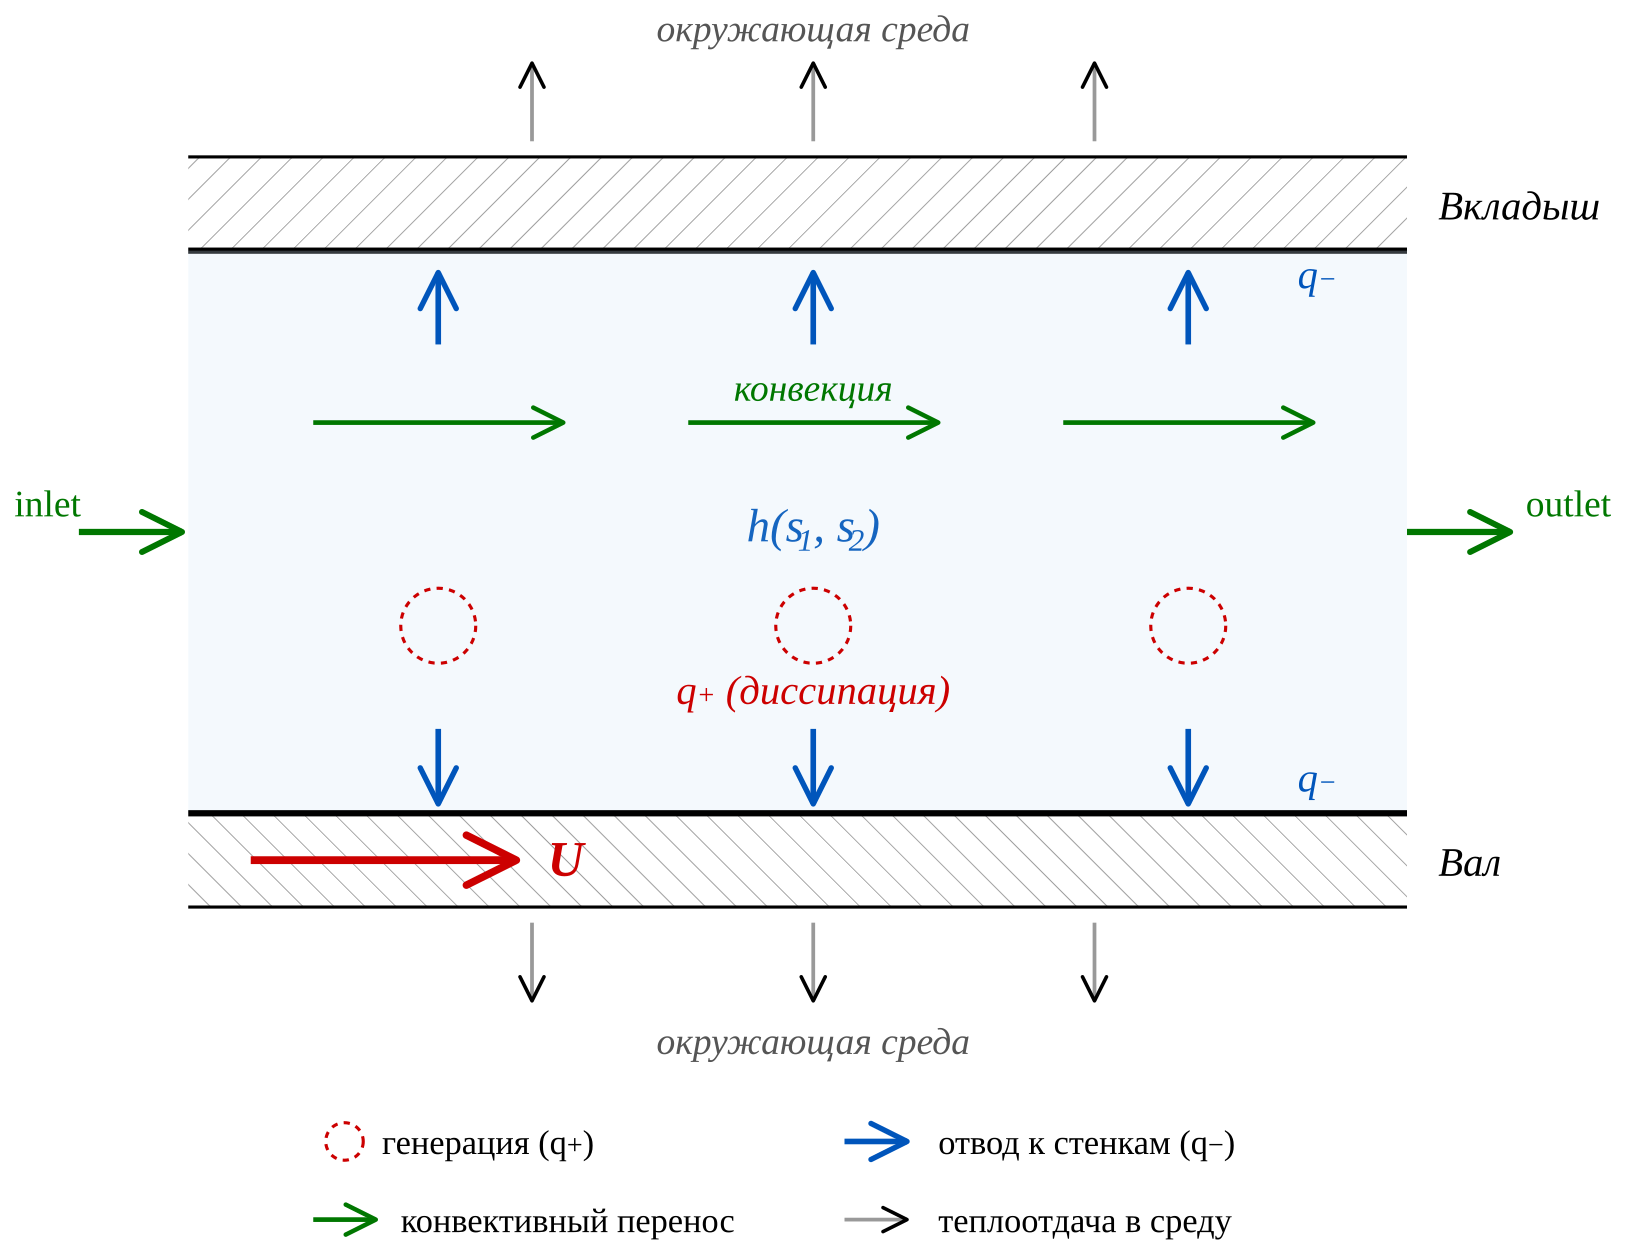
\includegraphics[width=\textwidth,height=0.9\textheight,keepaspectratio]{figures/ch04/fig_4_1.png}
\caption{Источники и каналы отвода теплоты в смазочном слое}
\label{fig:heat_balance}
\end{figure}

\FloatBarrier

\textit{Уровни учёта температуры.}
В зависимости от требуемой точности и вычислительных
ресурсов можно выделить три уровня учёта температуры,
представляющих собой «лестницу сложности» модели.

Первый уровень~-- изотермическое приближение ($T = T_0$,
$\mu = \mu_0 = \mathrm{const}$): температурное поле
не рассчитывается, вязкость принимается постоянной.
Это наиболее простая и распространённая постановка,
используемая в расчётах глав~5--7 настоящей монографии.

Второй уровень~-- приближение эффективной температуры:
сначала решается уравнение Рейнольдса (или задача JFO)
с текущим значением вязкости, затем по полученному полю
давления и скоростей оценивается суммарная диссипация,
вычисляется эффективная температура~$T_{\mathrm{eff}}$
(например, из интегрального теплового баланса), после чего
вязкость обновляется как $\mu(T_{\mathrm{eff}})$
и процедура повторяется до сходимости. Уравнение энергии
в явном виде не решается, что существенно упрощает
реализацию, однако снижает точность при выраженной
неоднородности температурного поля.

Третий уровень~-- термогидродинамика (THD): совместное
решение уравнения Рейнольдса (или задачи JFO) и уравнения
энергии для поля~$T(s_1, s_2, t)$ с учётом зависимости
$\mu(T)$. Этот подход обеспечивает наибольшую точность,
но требует значительных вычислительных затрат, поскольку
на каждой итерации необходимо решать дополнительную краевую
задачу для температуры. Далее в разделе формулируется именно
постановка THD.

\textit{Зависимость вязкости от температуры.}
Для количественного описания влияния температуры
на вязкость необходима аналитическая зависимость $\mu(T)$.
Наиболее употребительным в расчётах тонкоплёночных течений
является экспоненциальный закон:
\begin{equation}
  \mu(T) = \mu_0 \exp\!\bigl(-\beta\,(T - T_0)\bigr),
  \label{eq:viscosity_exp}
\end{equation}
\begin{conditions}
$\mu_0 = \mu(T_0)$ -- вязкость при референсной температуре~$T_0$;\\
$\beta$ -- температурный коэффициент вязкости, $\beta > 0$, K$^{-1}$.
\end{conditions}
При умеренных перепадах температуры (порядка десятков кельвинов)
экспоненциальный закон~\eqref{eq:viscosity_exp} даёт хорошее
приближение и удобен аналитически: производная
$\partial\mu/\partial T = -\beta\,\mu$ линейна по~$\mu$,
что упрощает линеаризацию при итерационном решении.

Для масел в широком диапазоне температур более точным
является трёхпараметрический закон Фогеля:
\begin{equation}
  \mu(T) = A \exp\!\left(\frac{B}{T - C}\right),
  \label{eq:viscosity_vogel}
\end{equation}
\begin{conditions}
$A$, $B$, $C$ -- эмпирические параметры, определяемые
аппроксимацией паспортных данных смазочного масла;\\
$T$ -- абсолютная температура, К.
\end{conditions}
Закон Фогеля~\eqref{eq:viscosity_vogel} лучше описывает
нелинейность кривой $\mu(T)$ при больших температурных
перепадах, однако его параметризация требует экспериментальных
данных. В обоих случаях зависимость $\mu(T)$ является гладкой
и монотонно убывающей~-- повышение температуры приводит
к уменьшению вязкости, что, в свою очередь, снижает несущую
способность и увеличивает утечки, создавая обратную связь
между тепловым и гидродинамическим полями (рисунок~\ref{fig:viscosity_temp}).

\begin{figure}[!ht]
\centering
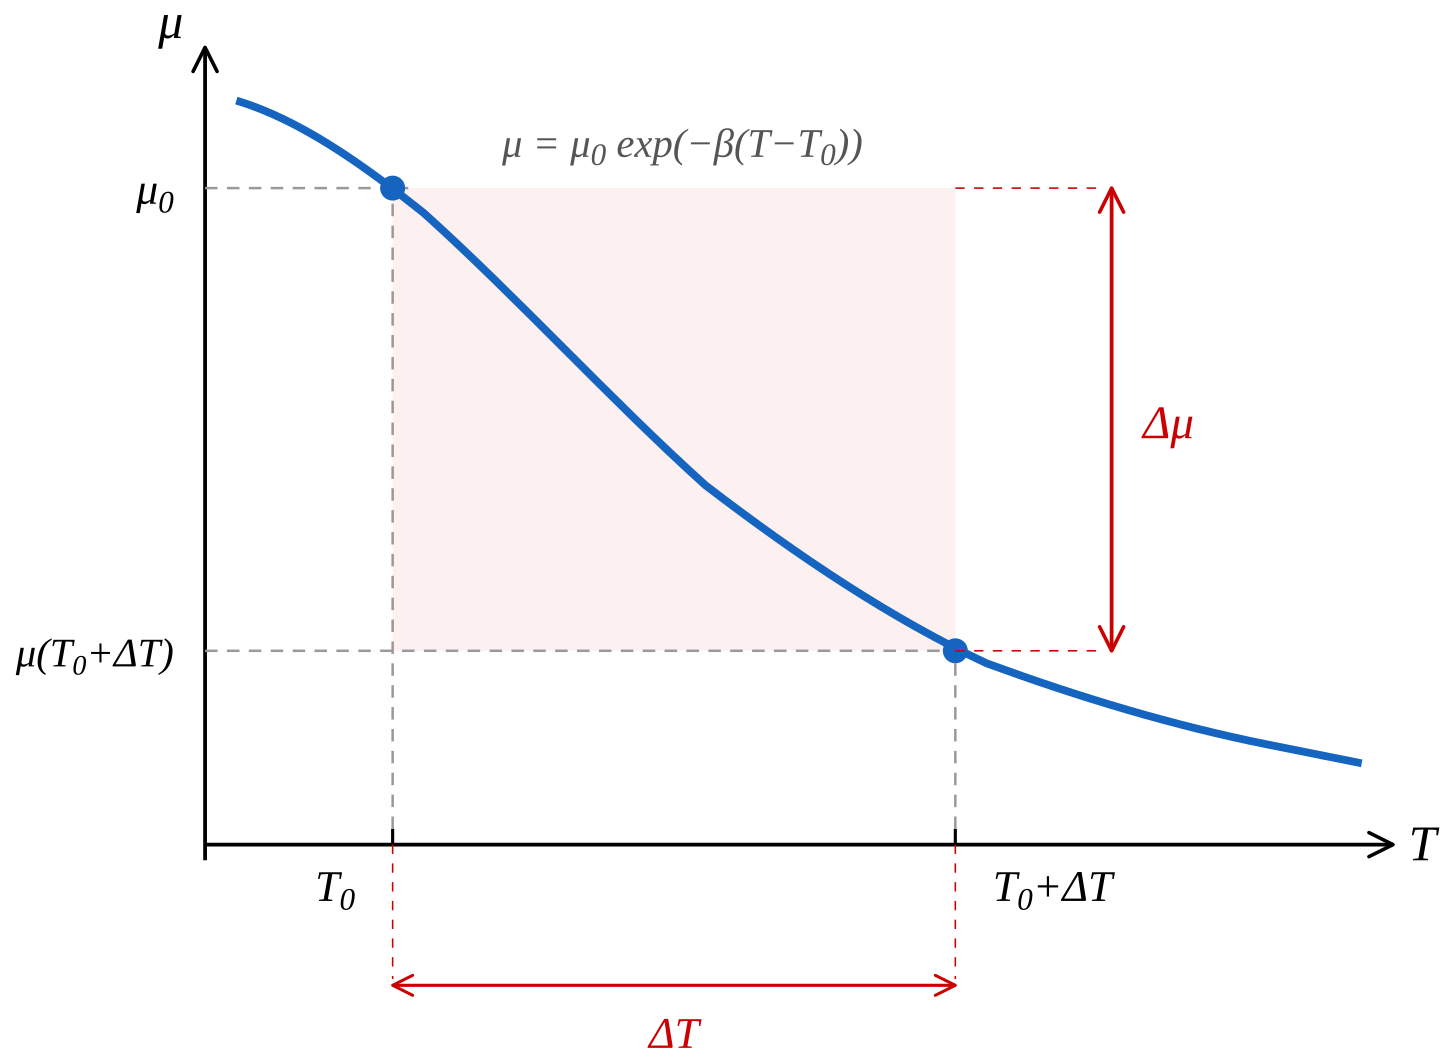
\includegraphics[width=\textwidth,height=0.9\textheight,keepaspectratio]{figures/ch04/fig_4_2.png}
\caption{Типовая температурная зависимость вязкости смазки}
\label{fig:viscosity_temp}
\end{figure}

\FloatBarrier

\textit{Уравнение энергии для смазочного слоя.}
Для описания температурного поля на третьем уровне учёта
(THD) необходимо уравнение энергии. Аналогично тому, как
в разделе~4.1 обобщение JFO с переменной плотностью
записывалось в размерной форме, уравнение энергии здесь
также приводится в размерных переменных. Используется
двумерная плёночная постановка, усреднённая по толщине
зазора:
\begin{equation}
  \rho\,c_p\,h\,\frac{\partial T}{\partial t}
  + \rho\,c_p\,h\,(\mathbf{u}_{\parallel} \cdot \nabla T)
  = \nabla\cdot(k_{\parallel}\,h\,\nabla T)
    + q^{+} - q^{-},
  \label{eq:energy_film}
\end{equation}
\begin{conditions}
$\mathbf{u}_{\parallel}$ -- средняя по толщине скорость
в плоскости $(s_1,\,s_2)$;\\
$c_p$ -- удельная теплоёмкость смазки при постоянном
давлении;\\
$k_{\parallel}$ -- эффективная теплопроводность смазки
в плоскости плёнки;\\
$q^{+}$ -- удельная мощность тепловыделения на единицу площади опорной поверхности, обусловленная вязкой диссипацией; оценка порядка: $q^{+} \sim \mu(T)\,U^2/h$;\\
$q^{-}$ -- удельная мощность теплоотвода на единицу площади к стенкам (валу и вкладышу).
\end{conditions}
Левая часть уравнения~\eqref{eq:energy_film} описывает
нестационарное накопление теплоты и её конвективный перенос
потоком смазки; правая часть~-- диффузию теплоты в плоскости
плёнки, генерацию за счёт диссипации и отвод к ограничивающим
поверхностям.

Средние по толщине скорости $\mathbf{u}_{\parallel}$ вычисляются по стандартным выражениям для тонкого слоя (суперпозиция куэттовского и пуазейлевского профилей) на основе полей $p$, $h$ и $\mu$, полученных на текущей итерации решателя.

\textit{Упрощённая конвективная модель как частный случай.}
В ряде практических постановок общее уравнение
энергии~\eqref{eq:energy_film} допускает существенное упрощение. Ниже приведён вариант для радиальной постановки, где $s_1 = \varphi$~-- окружная координата, $s_2 = Z = z/L$~-- безразмерная осевая координата, $H = h/c_0$~-- безразмерная толщина зазора, $c_0$~-- характерный радиальный зазор подшипника, $P$~-- безразмерное давление в соответствии с безразмеризацией подраздела~2.1.3.
Если принять стационарное приближение ($\partial T/\partial t = 0$),
пренебречь диффузией теплоты в плоскости плёнки
($\nabla\cdot(k_{\parallel}\,h\,\nabla T) \approx 0$) и считать,
что конвективный перенос теплоты осуществляется преимущественно
вдоль окружного направления~$\varphi$,
уравнение~\eqref{eq:energy_film} сводится к конвективной форме. В данной редуцированной постановке теплоотвод к стенкам явно не учитывается (формально $q^{-} \approx 0$); тепловой баланс замыкается конвективным переносом и условием частичного перемешивания на входе~\eqref{eq:bc_partial_mix}:
\begin{equation}
  \mathrm{Pe}\cdot H\,\frac{\partial T}{\partial\varphi}
  = Q_{\mathrm{total}}\cdot\Delta T_{\mathrm{ref}},
  \label{eq:energy_convective}
\end{equation}
где $\mathrm{Pe} = \rho\,c_p\,U\,c_0/k$~-- число Пекле,
характеризующее соотношение конвективного и кондуктивного переноса
теплоты ($k$~-- теплопроводность смазки); $H = h/c_0$~-- безразмерная толщина зазора;
$\Delta T_{\mathrm{ref}}$~-- опорный температурный перепад, используемый при безразмеризации уравнения энергии.
Уравнение~\eqref{eq:energy_convective} является рабочей формой
тепловой модели, реализованной в расчётном модуле.
Уравнение~\eqref{eq:energy_convective} представляет собой ОДУ по~$\varphi$ и решается численным интегрированием по окружности совместно с условием~\eqref{eq:bc_partial_mix}.

Безразмерный источник теплоты~$Q_{\mathrm{total}}$ объединяет вклады
вязкого сдвига (доминирующий) и напорного течения
(пропорциональный~$H^3$):
\begin{equation}
  Q_{\mathrm{total}} = \frac{1}{H}
  + \gamma\,H^3\!\left[
      \left(\frac{\partial P}{\partial\varphi}\right)^{\!2}
      + \left(\frac{D}{L}\right)^{\!2}
        \left(\frac{\partial P}{\partial Z}\right)^{\!2}
    \right],
  \label{eq:Q_total}
\end{equation}
где $P$~-- безразмерное давление; $D$,~$L$~-- диаметр и длина
подшипника; $\gamma$~-- коэффициент, определяемый выбранными
масштабами безразмеризации (в реализованной модели $\gamma = 0{,}1$).
Первое слагаемое~$1/H$ отражает сдвиговую диссипацию Куэтта, второй
член~-- дополнительный вклад пуазейлевской компоненты течения от
градиента давления.

Граничное условие на входе задаётся в виде частичного перемешивания
свежей смазки с нагретой после полного оборота:
\begin{equation}
  T\big|_{\varphi=0}
  = \tfrac{1}{2}\,T_{\mathrm{inlet}}
  + \tfrac{1}{2}\,T\big|_{\varphi=2\pi},
  \label{eq:bc_partial_mix}
\end{equation}
где $T_{\mathrm{inlet}}$~-- температура подаваемой свежей смазки.
Условие~\eqref{eq:bc_partial_mix} моделирует ситуацию, при которой
масло на входе в зазор представляет собой равную смесь свежего масла
и масла, прошедшего полный оборот; в результате эффективная
температура на входе оказывается выше~$T_{\mathrm{inlet}}$, что
соответствует реальному тепловому балансу в подшипнике с непрерывной
циркуляцией смазки.

В полной постановке~\eqref{eq:energy_film} теплоотвод к стенкам задаётся явно через~$q^{-}$; ниже приведены два типовых варианта. При известных температурах стенок используются условия первого рода:
\[
  T_{\mathrm{wall},1} = \mathrm{const}, \qquad
  T_{\mathrm{wall},2} = \mathrm{const},
\]
и~$q^{-}$ определяется из решения поперечного профиля
температуры. Альтернативный, более гибкий подход~-- задание
эффективного конвективного теплоотвода:
\[
  q^{-} = \alpha_1\,(T - T_{\mathrm{wall},1})
         + \alpha_2\,(T - T_{\mathrm{wall},2}),
\]
где $\alpha_1$,~$\alpha_2$~-- коэффициенты теплоотдачи,
определяемые условиями конкретной задачи (геометрией,
теплопроводностью материалов, режимом течения).

Граничные условия для уравнения~\eqref{eq:energy_film}
в плоскости~$(s_1, s_2)$ задаются следующим образом:
на входной границе смазочного слоя температура задана
($T = T_{\mathrm{in}}$), на выходной границе принимается
условие свободного выхода ($\partial T/\partial n = 0$).

\textit{Алгоритм термовязкостного итерационного цикла.}
Совместное решение уравнения Рейнольдса (или задачи JFO)
и уравнения энергии~\eqref{eq:energy_film} с зависимостью
$\mu(T)$ осуществляется итерационно. Структура алгоритма
совместима с двухуровневой схемой решения JFO, описанной
в разделе~3.5: температурный цикл выполняется как
дополнительный внешний уровень, охватывающий циклы
по давлению и кавитации. Последовательность шагов
на каждой итерации~$m$ выглядит следующим образом.
\begin{enumerate}[wide, labelindent=\parindent, nosep]
  \item Задать начальное поле
    $T^{(0)} = T_0$ и вычислить начальную вязкость
    $\mu^{(0)} = \mu(T_0)$.
  \item Решить уравнение Рейнольдса или задачу JFO
    с текущим полем вязкости~$\mu^{(m)}$; получить
    давление~$p^{(m)}$ и поле скоростей.
  \item Решить уравнение энергии~\eqref{eq:energy_film}
    с источником~$q^{+}$, определённым по~$p^{(m)}$
    и~$\mu^{(m)}$; получить обновлённое
    поле~$T^{(m+1)}$.
  \item Применить релаксацию по температуре:
    $T^{(m+1)} \leftarrow (1 - \omega_T)\,T^{(m)}
    + \omega_T\,T^{(m+1)}$,
    где $\omega_T \in (0,\,1]$~-- параметр релаксации;
    после релаксации обновить вязкость:
    $\mu^{(m+1)} = \mu(T^{(m+1)})$ по
    закону~\eqref{eq:viscosity_exp}
    или~\eqref{eq:viscosity_vogel}.
  \item Проверить критерии сходимости; при их выполнении
    остановиться, в противном случае вернуться к шагу~2.
\end{enumerate}

Критерии сходимости формулируются по отклонениям полей
температуры и давления между последовательными итерациями:
\begin{equation}
  \|\,T^{(m+1)} - T^{(m)}\| < \varepsilon_T, \qquad
  \|\,p^{(m+1)} - p^{(m)}\| < \varepsilon_p.
  \label{eq:thd_convergence}
\end{equation}

Параметр релаксации~$\omega_T$ выбирается из условия
устойчивости итераций; при сильной зависимости~$\mu(T)$
(больших значениях~$\beta$ в~\eqref{eq:viscosity_exp})
может потребоваться умеренная подрелаксация
($\omega_T = 0{,}3\text{--}0{,}7$). Важно отметить, что
описанный алгоритм совместим с кэшированием GPU-буферов
(раздел~3.4): при обновлении~$\mu$ на каждой итерации
достаточно пересчитать коэффициенты дискретизации без
переразмещения памяти на устройстве.

\textit{Тепловые эффекты при наличии микроструктур.}
Микроструктуры поверхности существенно модифицируют
тепловую картину смазочного слоя по сравнению с гладким
зазором. Впадины и ячейки микрорельефа создают локальные
зоны с повышенным градиентом скорости сдвига: поскольку
удельная мощность диссипации пропорциональна $\mu\,U^2/h$,
в местах минимального зазора~-- у краёв и на гребнях ячеек~--
источник~$q^{+}$ возрастает резко и нелинейно. При гладком
зазоре диссипация распределена по полю относительно
равномерно; при наличии микротекстур возникают локальные
«горячие пятна», где температура может существенно превышать
среднюю по плёнке (рисунок~\ref{fig:hotspots_texture}).

\begin{figure}[!ht]
\centering
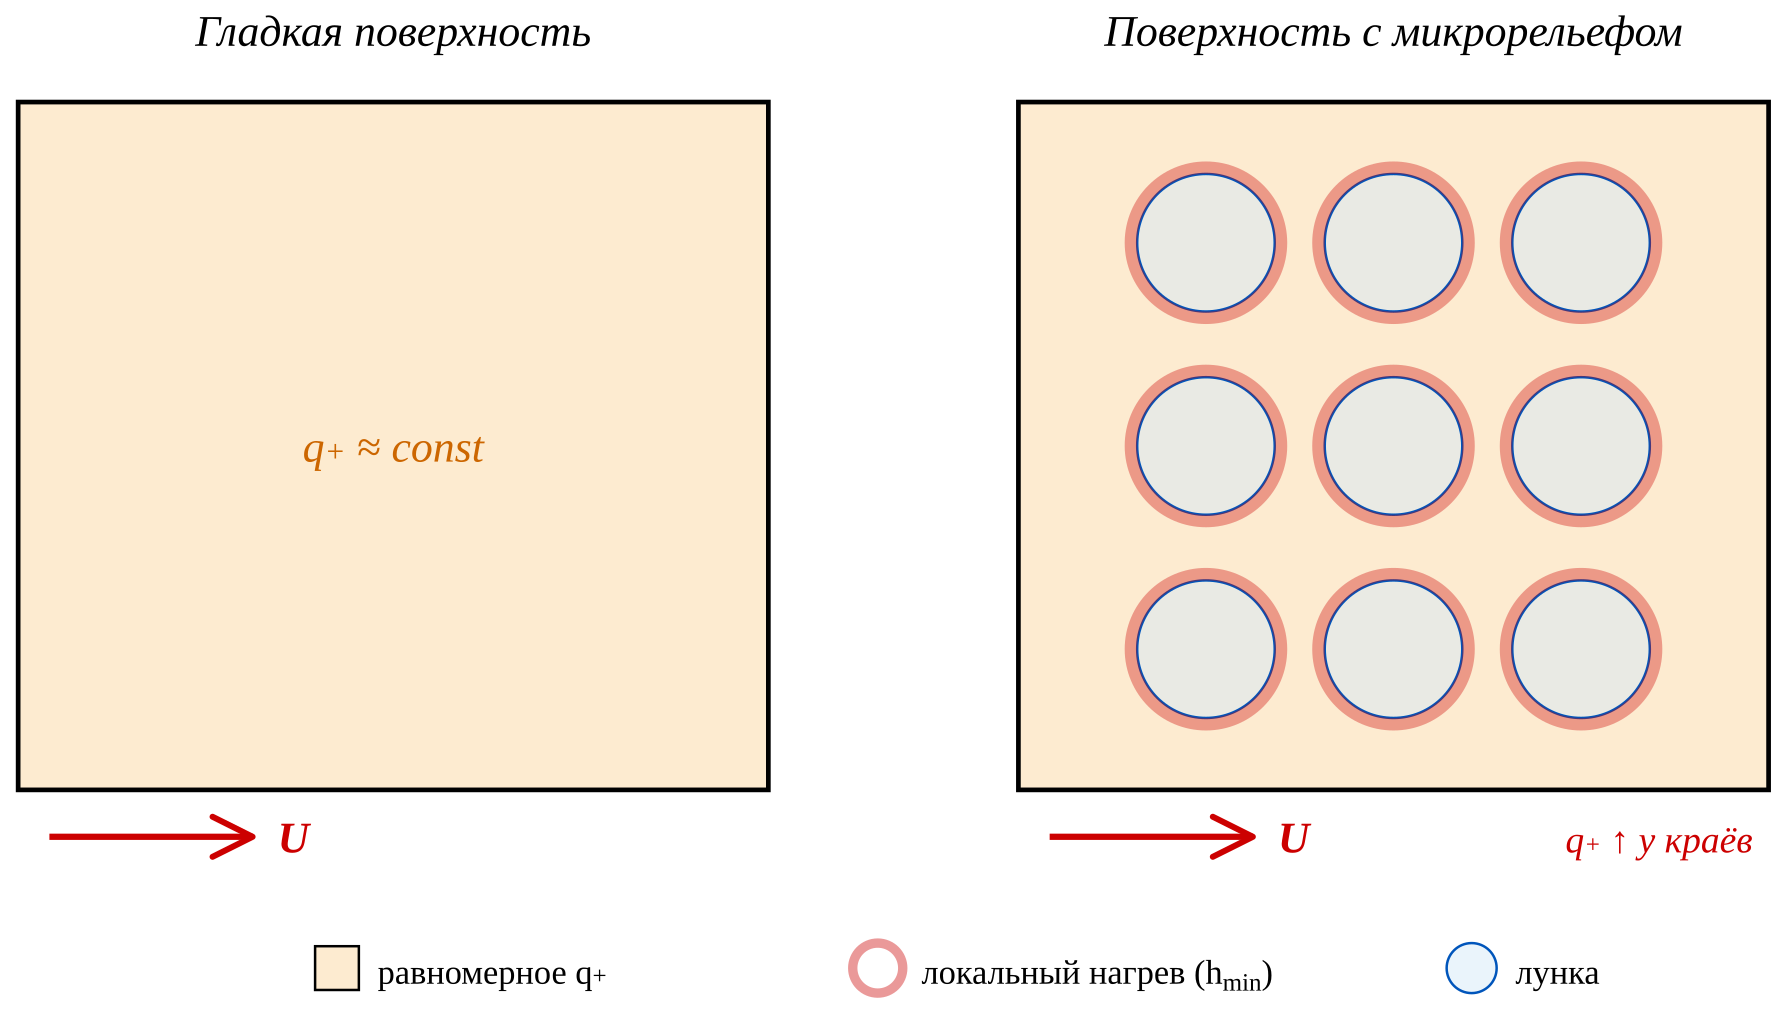
\includegraphics[width=\textwidth,height=0.9\textheight,keepaspectratio]{figures/ch04/fig_4_3.png}
\caption{Локализация диссипации при наличии микротекстур (схема):
  гладкая поверхность (слева) и поверхность с микрорельефом (справа)}
\label{fig:hotspots_texture}
\end{figure}

\FloatBarrier

Это означает, что средняя температура смазочного слоя может
оставаться умеренной, тогда как локальный нагрев в зонах
микрорельефа оказывается значительным и способен повлиять
на несущую способность и границы кавитации. Для корректного
описания таких эффектов необходимо разрешение расчётной
сетки, достаточное для детального представления каждой ячейки
микрорельефа; это требование согласуется с требованиями
по разрешению кавитационных зон, сформулированными
в разделе~4.1. Кавитация (степень заполнения $\vartheta < 1$)
дополнительно модифицирует перенос теплоты в двухфазной
зоне~-- снижение плотности и теплоёмкости газожидкостной
смеси изменяет баланс
уравнения~\eqref{eq:energy_film}; в рамках настоящего
раздела этот эффект детально не раскрывается, однако
представляет собой направление возможного расширения модели.

В расчётах глав~5--7 используется изотермическое
приближение: $T = T_0$, $\mu = \mathrm{const}$. Такой подход
оправдан при умеренных скоростях скольжения и нагрузках, когда
температурный перепад в слое мал и его влияние на вязкость
несущественно. Постановка THD, изложенная
в настоящем разделе, обеспечивает основу для расширения модели
в случаях, когда тепловые эффекты становятся определяющими~--
в частности, при высоких скоростях скольжения, использовании
вязких масел или при глубоких микроструктурах с локально
высокой диссипацией~\cite{kyrkou2020,pierre2004,sun2010,talaighil2015}.
